
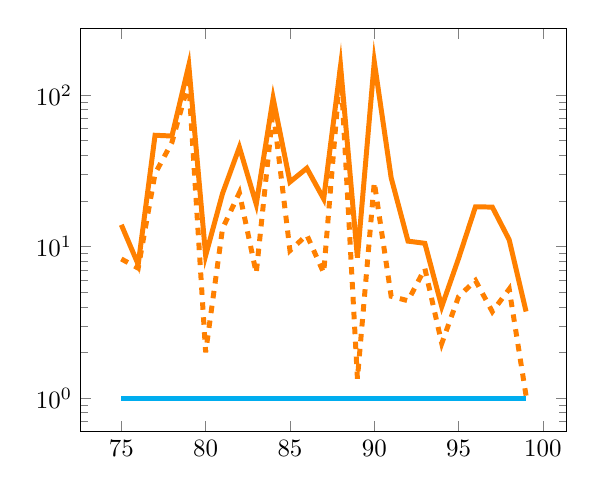
\begin{tikzpicture}[scale=0.9]
\begin{semilogyaxis}
\addplot[color=cyan,line width=2pt] coordinates {(75,1.0)(76,1.0)(77,1.0)(78,1.0)(79,1.0)(80,1.0)(81,1.0)(82,1.0)(83,1.0)(84,1.0)(85,1.0)(86,1.0)(87,1.0)(88,1.0)(89,1.0)(90,1.0)(91,1.0)(92,1.0)(93,1.0)(94,1.0)(95,1.0)(96,1.0)(97,1.0)(98,1.0)(99,1.0)};
\addplot[color=orange,line width=2pt] coordinates {(75,13.91874783245831)(76,7.617443612970986)(77,54.27207914677402)(78,53.66313134120323)(79,157.3648974107742)(80,8.720076270740703)(81,22.38223334146772)(82,45.237081844975854)(83,19.041575458324953)(84,95.40290374470739)(85,26.69389597998642)(86,32.89475580176832)(87,20.62911705542232)(88,155.70840073374413)(89,8.43450213581268)(90,165.83625816205472)(91,28.44981295024453)(92,10.860217443810495)(93,10.503667218777847)(94,4.012842999757378)(95,8.358623159248125)(96,18.291034917702067)(97,18.21886904544698)(98,11.077179110464703)(99,3.7256748443679912)};
\addplot[dashed,color=orange,line width=2pt] coordinates {(75,8.279035099329487)(76,7.20293343836156)(77,30.28410252932198)(78,48.707499775532625)(79,121.244059575766)(80,2.0035929360711684)(81,13.144212463893012)(82,22.66444721817792)(83,6.680787483025451)(84,80.16035882694447)(85,9.406865609044145)(86,11.929046365817754)(87,6.698844517257057)(88,154.953161695919)(89,1.3403191656095708)(90,26.575049586460764)(91,4.696662843569498)(92,4.3873788940738985)(93,7.153955906303368)(94,2.293016622580435)(95,4.678773804108987)(96,5.970684480446588)(97,3.718053140263493)(98,5.240711140970649)(99,1.0353205703064787)};

\end{semilogyaxis}
\end{tikzpicture}
